\documentclass[12pt]{article}
\usepackage[left=3cm, right=2cm, top=2cm, bottom=2cm]{geometry}

\usepackage[english]{babel}				% orthography
\usepackage[T1]{fontenc}
\usepackage{times}				% font family
\usepackage{microtype}				% for micro typography (for a better typeface)
\usepackage{setspace}
\setstretch{1.5} % 1.5 line spacing
\newtheorem{mydef}{Merksatz}  		% if examples or mnemotechnic verses are used with continuous numeration
\newtheorem{bsp}{Beispiel}
\usepackage{blindtext}
\usepackage{fancyhdr}
\usepackage{longtable}
\usepackage{multicol}
\usepackage{multirow}
\usepackage{booktabs}
\usepackage{tabularx}
\usepackage{xcolor}
\usepackage{varioref}
\usepackage[active]{srcltx}
\usepackage{listings}				% algorithm
\usepackage{mdwlist}				% lists
\usepackage{calc}
\usepackage{tablefootnote}			% footnotes in tables
\hyphenation{voll-st\"andigen}		% for defining word devisions globally

\usepackage[utf8]{inputenc}
\usepackage{amsmath}

\usepackage{wrapfig}
\usepackage{array}  % For better control over column formatting

\usepackage{graphicx}
\graphicspath{{./Graphics/}}          % path to the pictures

\usepackage[hidelinks]{hyperref}
\hypersetup{colorlinks=true,
   linkcolor=blue,
   filecolor=magenta,
   urlcolor=cyan,
   citecolor=blue,
   pdfborderstyle={/S/U/W 0}
}

\usepackage[round]{natbib}
\bibliographystyle{plainnat}

\begin{document}

% Title page shall not include header or foooter lines
\thispagestyle{empty}

% All elements shall be centered
\begin{center}

    \vspace*{-8mm}

    {\LARGE INSTITUTE OF FINANCE AND STATISTICS\\[1mm]}
    \large University of Bonn\\

    \vspace*{1cm}

    
\includegraphics[width=0.4\textwidth]{./Graphics/UNI_Bonn_Logo_Standard_RZ.eps}

    \vspace*{1cm}

    % Kind of Thesis => (Bachelor Thesis ,Diploma Thesis, Master Thesis, Seminar Thesis)
    {\Large \textbf{Seminar Paper in Academic Practice}}\\

    \vspace{1cm}

    % Title of the Thesis
    {\Large \textbf{Regression Trees}}\\
    \vspace{1.5cm}

    % Names of Authors
    {\LARGE Timothy Currie}\\[15mm]

    % Superverisor, contact data and submission date
    \parbox{120mm} {
        \begin{large}
            \begin{tabbing}
                Supervisor: \hspace{1.8cm} \= Dr. Elias Wolf\\[1.5mm]
                Semester:\> Summer Term 2024\\[1.5mm]
                Author:\>Timothy Jakob Currie\\[1.5mm] % alphabetic order (Surname)
                Matriculation-Nrs.:\> 50074426\\[1.5mm]
                %Address:\> Street Nr, Postal Code City\\[1.5mm]
                Email:\> s69tcurr@uni-bonn.de\\[1.5mm]
                Subject:\>Bachelor Economics\\[1.5mm]
                Submission:\> 25. August 2024\\[1.5mm]
            \end{tabbing}
        \end{large}
    }

\end{center}
\clearpage{\pagestyle{empty}\cleardoublepage}


\pagenumbering{arabic}% Arabic and reset to 1

\tableofcontents

%\newpage

\section{Introduction}

A large part of modern economic research is built upon linear regression. To conduct and understand economic research, it is particularly crucial to identify where it performs well and where its limitations lie and other methods can improve upon it. Regression trees are a powerful machine-learning technique, that can be useful in many situations where linear regression falls short. Particularly for data that includes non-linear relationships and interaction effects linear regression will often perform poorly. And regression trees can be an important alternative. Regression trees also have numerous extensions that greatly improve their usefulness and applicability.

The CART algorithm or variations on it, that most tree based methods use was first introduced in \citep{breiman1984}. Since then many extensions have been developed such as Random forests, a very popular tree based ML method. \citep{biau2016} serves as a good introduction to that method. \citep{hastie2021} serves as an excellent modern introduction to regression trees and gives a gentle introduction to the topic and many extensions. \citep{tan2019} give a deeper dive on Bayesian additive regression trees (BART), one powerful ensemble method.

In this paper I will explain the theory behind regression trees and compare them to linear regression using a series of simple simulations and on a dataset of student test performance. Simulations can allow for comparison under ideal circumstances, allowing one to focus on the issue one is interested in, while real world data can give a more realistic perspective on a methods actual performance. I will focus especially on the regression trees ability to naturally capture interaction effects, and how pruning can combat overfitting. I will also highlight how ensemble methods, a kind of extension to regression trees, can enhance their performance substantially.

In section 2 I will give a brief overview of the theory of regression trees, and where and where not one might expect them to perform well. And will also explain the bias-variance trade-off and explain how pruning helps and ensemble methods that are extensions to trees. In section 3 I will run a number of simulations comparing the performance of linear regression and regression trees under ideal conditions. In section 4 I will apply these methods to a dataset of student test performance. Highlighting pruning and the BART ensemble method. Also showing some of the shortcomings of regression trees. Section 5 is the conclusion and will sum up what I have found and further interesting areas where research could be done.

This dataset used in this paper is publicly available at \href{https://www.kaggle.com/datasets/uciml/student-alcohol-consumption}{Kaggle: Student Alcohol Consumption Dataset}. All code used for the simulations and data analysis is available at \href{https://github.com/Tim2othy/wissenschaftliches-arbeiten}{my GitHub}.


\section{Regression Trees}

Regression trees are a type of supervised machine-learning algorithm that recursively splits the predictor space into smaller rectangular subregions. This process approximates an unknown function $f$ by minimizing a measure of loss at each split. Unlike linear regression, regression trees do not make assumptions about linearity or non-interaction between different dimensions, making them particularly useful for complex, non-linear relationships in data.

The core mechanism of regression trees involves splitting the predictor space into regions that minimize the residual sum of squares, given by:

\begin{equation}
    \sum_{j=1}^{J} \sum_{i \in R_j} ( y_i- \hat{y}_{R_j})^2
\end{equation}

In each region, $\hat{y}$ typically takes on the mean of all observations in that region. Each branching of the tree divides the predictor space into one extra reason, for numerical variables typically of the form $\{x \le c\}$ or $\{x > c\}$. This process continues until a specified threshold is reached, such as a minimum number of observations in each leaf node or a maximum tree depth. Figure~\ref{red_visual} shows one way to visualize the way a regression tree will carve up the predictor space and make predictions for each region.

The algorithm employs a greedy approach called Recursive binary splitting to find the optimal split at each stage to minimize prediction error.

\begin{wrapfigure}{r}{0.5\textwidth}
    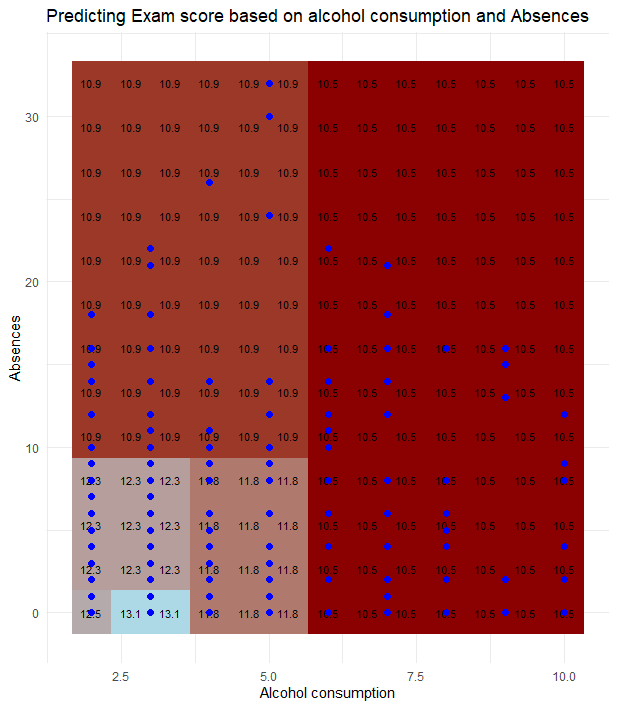
\includegraphics[scale=0.40]{red_visual.png}
    \caption{Visualization of regression trees predictions}
    \label{red_visual}
\end{wrapfigure}

Regression trees offer several advantages over traditional linear regression methods.  Furthermore, they naturally account for interaction effects. For instance, if, in one's dataset, being tall increases income but only for men, a regression tree will naturally partition the data along gender and only along hight for the male half. Whereas for a linear regression to capture this interaction effect would require one to explicitly include this interaction on one of one's regressors. This ability to model complex interactions without manual specification is a significant strength of the method.

One major weakness of regression trees however is their tendency to overfit on the data. To capture interesting relationships one must allow one's tree to grow deep with multiple levels of splits. Their flexibility allowing them to create very specific rules also allows them to capture noise in the training data rather than true underlying patterns. Figure~\ref{overfitting_tree}, illustrates how a regression tree can overfit a dataset.

\begin{figure}
    \centering
    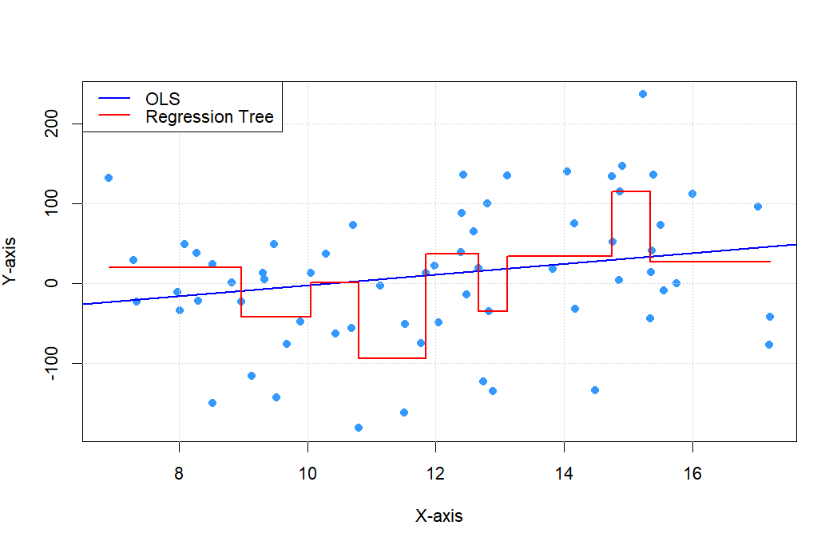
\includegraphics[scale=0.50]{image.png}
    \caption{Regression tree overfitting}
    \label{overfitting_tree}
\end{figure}


\subsection{Pruning}

The main way to address the overfitting problem is to, in keeping with the arboreal theme, "prune" one's regression tree. In cost complexity pruning one starts by growing a large tree that is bound to overfit the training data. Then, a complexity parameter $\alpha$ is introduced to penalize the trees size. The pruning process is guided by the following formula:

\begin{equation}
    \sum_{m=1}^{|T|} \sum_{i: x_i \in R_m} (y_i - \hat{y}_{R_m})^2 + \alpha|T|
\end{equation}

Where $|T|$ is the number of terminal nodes in the tree. The tree shrinks in a predictable fashion as the cost complexity parameter $\alpha$, is increased and it becomes harder for each split to justify its existence. As one prunes a large tree by increasing $\alpha$, the tree naturally shrinks in a well-behaved fashion, allowing one to select the subtree with the lowest cross-validation error. Evaluating a model on different data than it was trained on allows us to see its real performance and select a subtree that achieves a good trade-off between bias and variance. In the \texttt{rpart} library cross-validation is performed automatically each time one grows a tree.


\subsection{Ensemble Methods}
While pruning can improve the performance of regression trees, they often still underperform compared to other machine-learning methods. This has lead to the development of a number of ensemble methods, which combine many regression trees to create more robust and accurate predictions. As the well know jury theorem shows, if predictors are (sufficiently) uncorrelated and a predictors answer is better than pure chance adding more predictors will increase the quality of the average of all answers \citep{condorcet1785}. Ensemble methods leverage this "wisdom of crowds" effect.

Two ways this can be done is by Growing many independent trees and averaging them. Random forests are a very popular ML method that does this. Or by iteratively growing trees on the residuals of the current model, improving the overall model over multiple generations, as in boosting or BART.

Random forests create an ensemble by growing many decorrelated trees. Each tree is trained on a random subset of the training data and is only allowed to consider a random subset of features at each split. The final prediction is then formed by averaging the predictions of all trees, typically around 500. This approach reduces overfitting while maintaining the ability to capture complex patterns in the data \citep{biau2016}.

I will go into slightly more detail for the BART method, the method I used on the dataset. BART model the data as a sum of many trees plus noise:

\begin{equation}
    Y_i = \sum_{j=1}^{m} g(X_i; T_j, M_j) + \epsilon_i
\end{equation}

Where $m$ is the number of trees, typically around 200. And $g(X_i; T_j, M_j)$ represents the contribution of the $j$-th tree. $T_j$ and $M_j$ represent the trees structure and predictions respectively.

BART employs a Bayesian approach, incorporating a prior that discourages trees from growing too large. Specifically, the probability that a node at depth $d$ is non-terminal is given by $\alpha(1 + d)^{-\beta}$. This prior on shallow trees, restricts the trees to be weak learners that only explain a small portion of the overall data and are better suited to being combined through summation and averaging. In doing this BART avoids overfitting and leverages the strengths of ensemble learning. Additionally, BART employs other priors to guide the estimation of terminal node parameters, though a detailed discussion of these is beyond the scope of this paper. This Bayesian approach enables the model to provide both accurate predictions and quantitative measures of uncertainty.

Default values for these hyperparameters of $\alpha = 0.95$ and $\beta = 2$ are recommended by \citep{chipman2010}. And generally provide good performance.

The BART algorithm proceeds by first generating e.g., 200 trees, without any splits. For each tree $j$, considering all the current trees except $j$, the residual error $R_{-j}$ is calculated:

\begin{equation}
    R_{-j} = Y - \sum_{t\not=j} g(X,T_j,M_j).
\end{equation}

Then a change to that trees structure is proposed, such as pruning or growing a node, or changing a splitting rule, and is accepted or rejected based on its posterior probability. Meaning the split has to be in accordance with the model parameters as well as fit the data well enough. This process is repeated for all $m$ trees. That constitutes one iteration of the algorithm. Typically, BART uses 1000 burn-in iterations followed by 1000 sampling iterations. An estimate for $f(x)$ is obtained by taking the average over all sample iterations.

A more complete exposition can be found in \citep{tan2019} or \citep{chipman2010}.

Ensemble methods have demonstrated remarkable success across various applications, often surpassing individual regression trees and many other machine learning techniques.


\section{Simulations}

Simulations can serve as a testing ground for statistical methods, allowing for easier repeatability and eliminating many of the complications that arise when using datasets. Simulations are especially useful in comparing two different methods. In this section I will compare linear regression and regression trees on linear and non-linear simulated data, each simulation having been run 400 times to average out noise. The regression trees were limited to four terminal nodes for both simulations.

\begin{wrapfigure}{r}{0.5\textwidth}
    \centering
    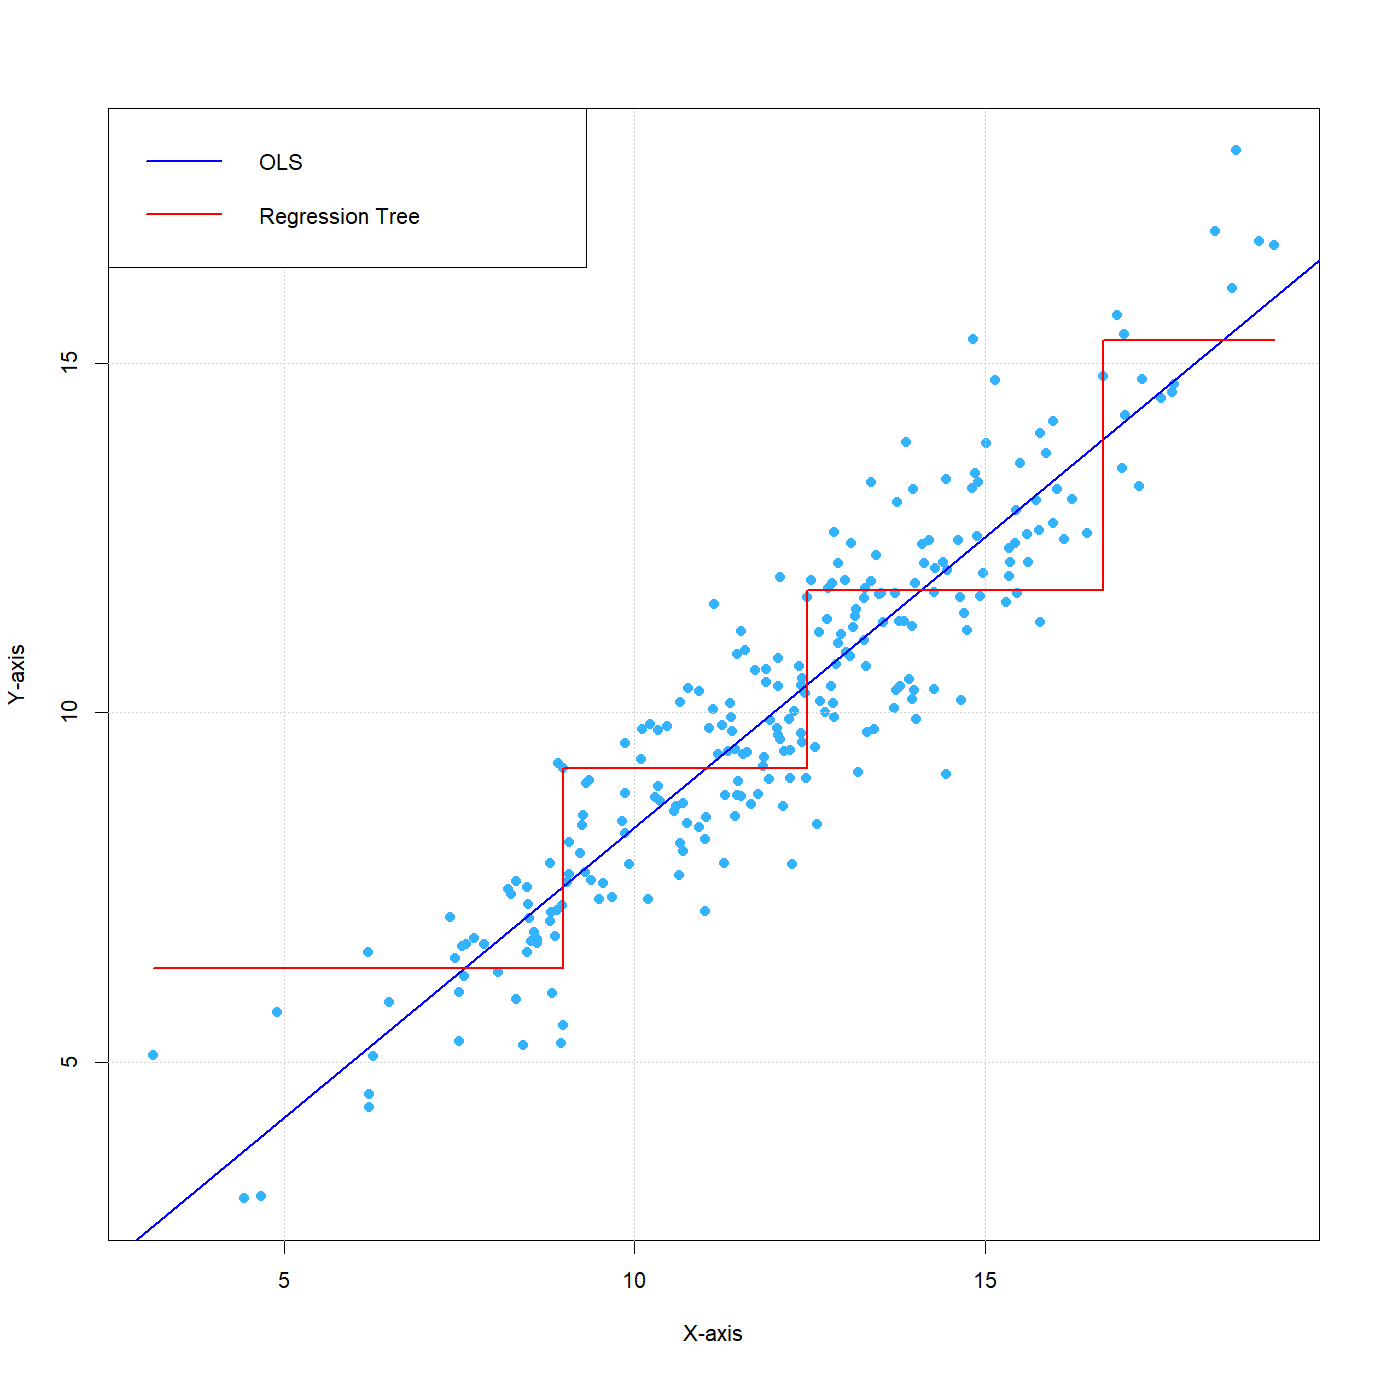
\includegraphics[scale=0.25]{OLS vs Tree.png}
    \caption{On linear Data}
    \label{OLS_VS_TREE}
\end{wrapfigure}

For the first simulation the data follow a simple linear relationship with $Y = \beta_0 + \beta_1X + \epsilon$, with $\epsilon$ normally distributed. For this simulation the mean squared error (MSE) for the linear regression is \texttt{0.992} and \texttt{1.494} for the tree. Figure~\ref{OLS_VS_TREE} shows quite clearly that this is the kind of data where it will be hard to beat linear regression.

The linear regression also wins out on intuitiveness. The derivative of the line of best fit can be interpreted as the expected increase in variable $y$ as the $x$ variable increases. While the trees step function lacks this.

In this second simulation, the data have a non-linear relationship. The data was generated using 4 normal distributions with varying variance, in the four corners of a two dimensional space. With the datapoints of the North-West and South-East distributions coloured in red and the North-Eastern and South-Western points in blue.

\begin{figure}
    \centering
    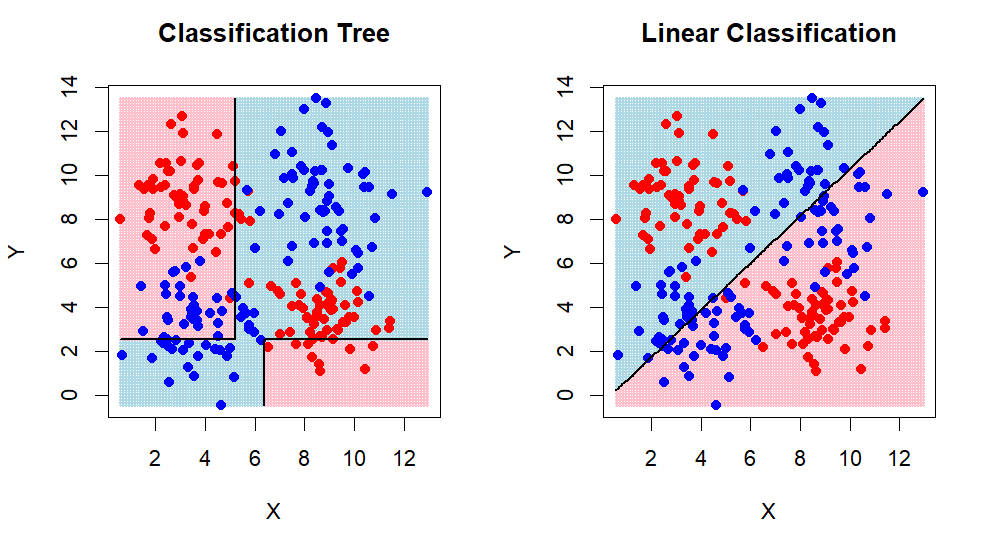
\includegraphics[scale=0.30]{NLD Pred.png}
    \caption{On non-linear Data}
\end{figure}

Using classifiers instead of regressors for this simulation the error rates of the tree and linear classifier are 37.57\% and 51.03\% respectively. The interaction effect between the two dimensions is not captured by the linear model, while the regression trees naturally captures it.


\section{Empirical Application}

Next, I will apply tree-based methods and also linear regression to a dataset to showcase differences in a more realistic situation. This dataset of student performance includes 649 students and looks at 33 variables.


\subsection{Pruning}

For all experiments on the dataset, I split the data into training (70\%) and validation (30\%) sets.

To prevent overfitting and ensure meaningful insights, it is crucial to use cross-validation and prune the regression tree. Without pruning, the model risks fitting to noise in the data, leading to misleading conclusions. While one will generally want to use the built-in automatic pruning, manually pruning trees can provide valuable intuition about how regression trees tend to overfit. Instead of relying solely on the built-in 10-fold cross-validation to automatically select the optimal tree, I first experimented with manual pruning.

By growing a large tree with a complexity parameter of \( \text{cp} = 0.01 \), I obtained a tree with a training Mean Squared Error (MSE) of 4.521 and a test error of 9.027, clearly indicating overfitting with the large tree. A smaller tree grown with \( \text{cp} = 0.025 \) resulted in a training MSE of 7.841 and a only slightly worse test error of 8.651.

\begin{wrapfigure}{r}{0.5\textwidth}
    \centering
    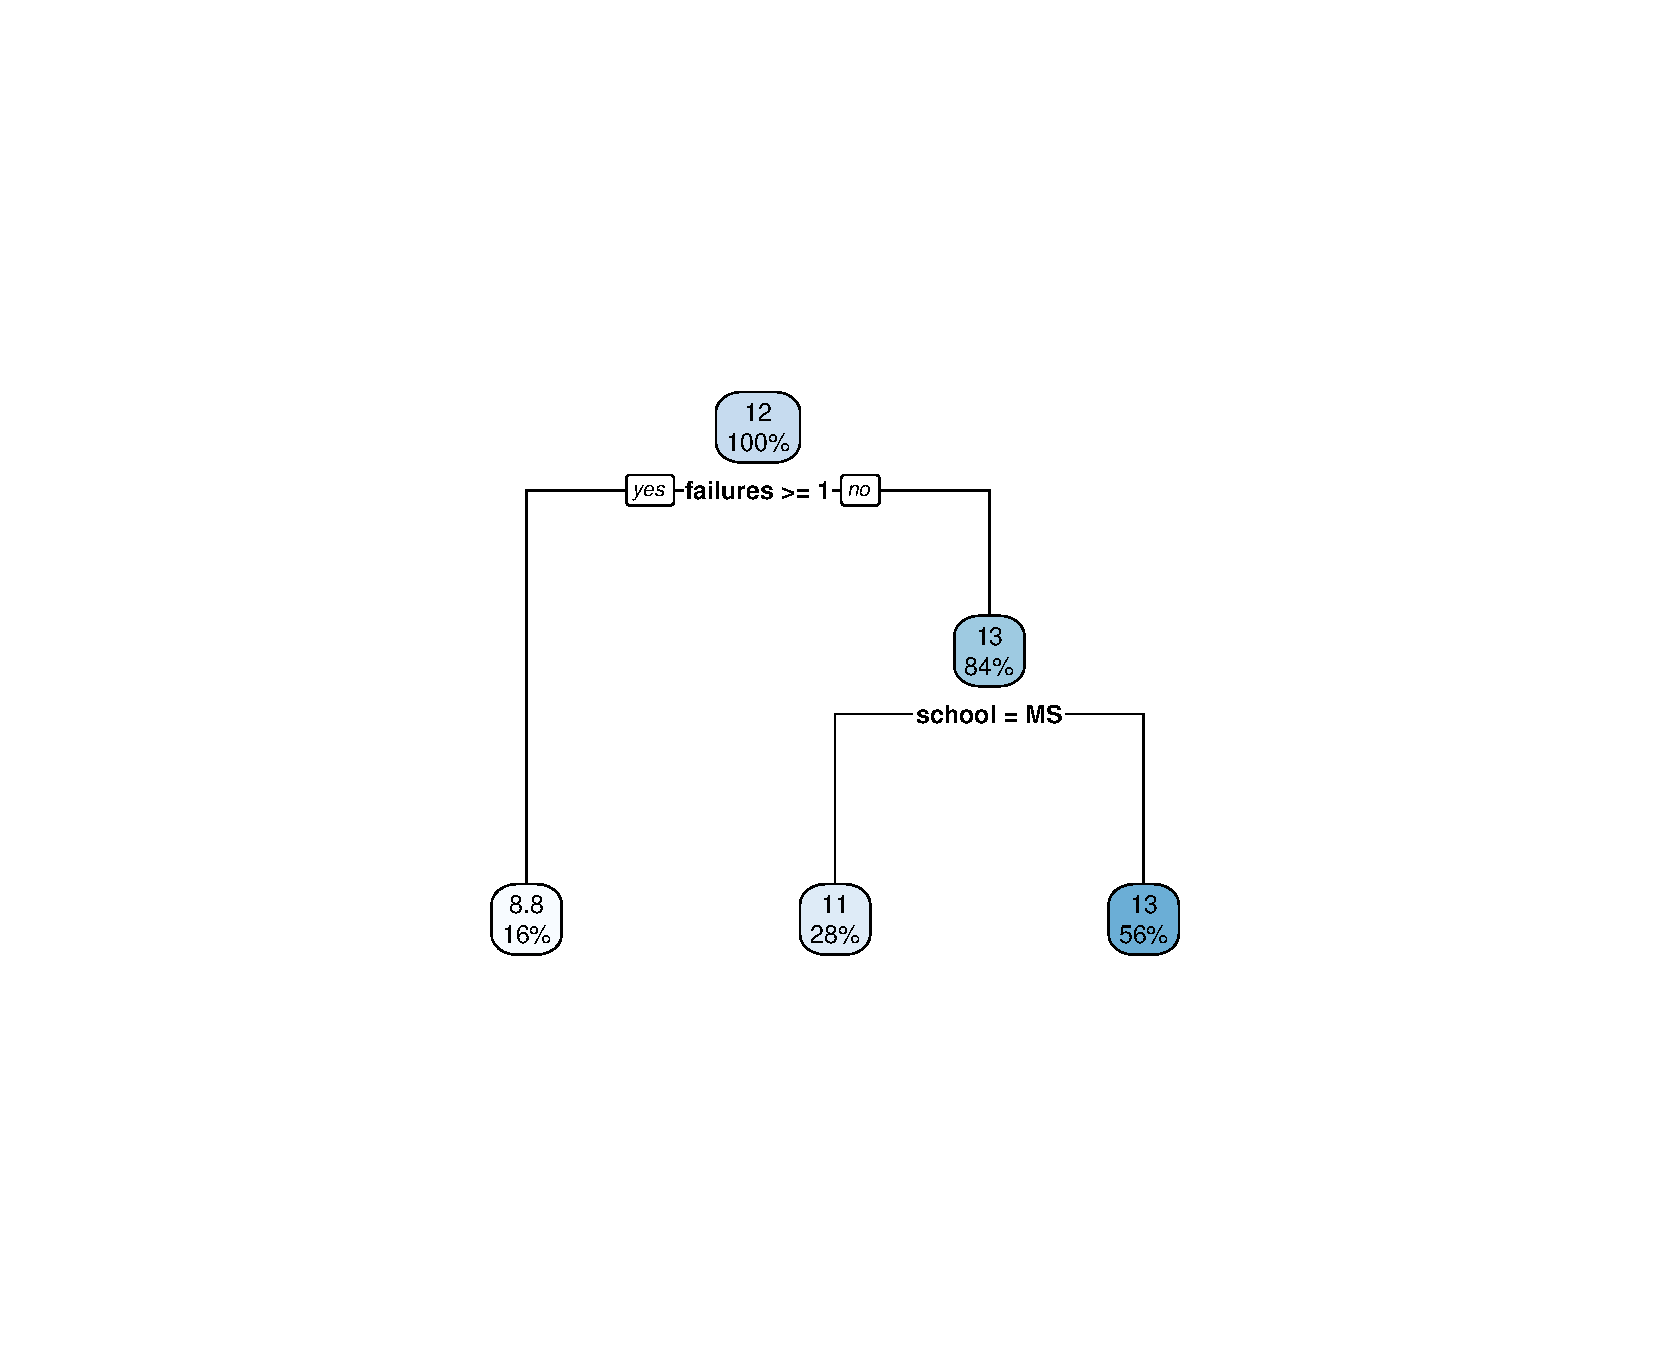
\includegraphics[scale=0.30]{small_manual_tree.pdf}
    \caption{Smaller, better tree}
    \label{small_tree}
\end{wrapfigure}

While it may seem counterintuitive that this simpler tree (Figure~\ref{small_tree}) outperforms the larger one, the larger tree fits the noise rather than the underlying signal, which explains its poor performance.

To find the best tree, one should employ proper automatic pruning using cross-validation. However, simply going with the optimal tree chosen using cross-validation is often insufficient to avoid overfitting. It can happen that a particular subtree coincidentally performs very well on the validation set and achieves a very low cross-validation error. Because many different subtrees are being evaluated, one can be very good merely by chance.

To mitigate this, it is important to use separate validation and test sets, not allowing oneself to experiment around with the test set until one finds a tree that happens to perform especially well on it by chance.

When evaluating the trees using a separate test set, in this case, the optimal pruned tree ends up making just one split, separating 15\% of students who had failed the exam before from the students who had no failures.

\begin{wraptable}{r}{0.5\textwidth}
    \centering
    \begin{tabular}{| l | c | c |}
        \hline
        Model        & Training MSE & Test MSE \\
        \hline
        Complex tree & 1.715        & 10.813   \\
        Pruned tree  & 8.527        & 8.189    \\
        \hline
    \end{tabular}
    \caption{MSE values for different models}
    \label{table_pruning}
\end{wraptable}

Typical test errors are shown in Table~\ref{table_pruning}. It is not surprising that the test error is lower than the training error for the pruned tree; with only one split, the tree could not overfit even if it tried, so any difference in error between the training and test sets is due to chance.

\begin{figure}
    \centering
    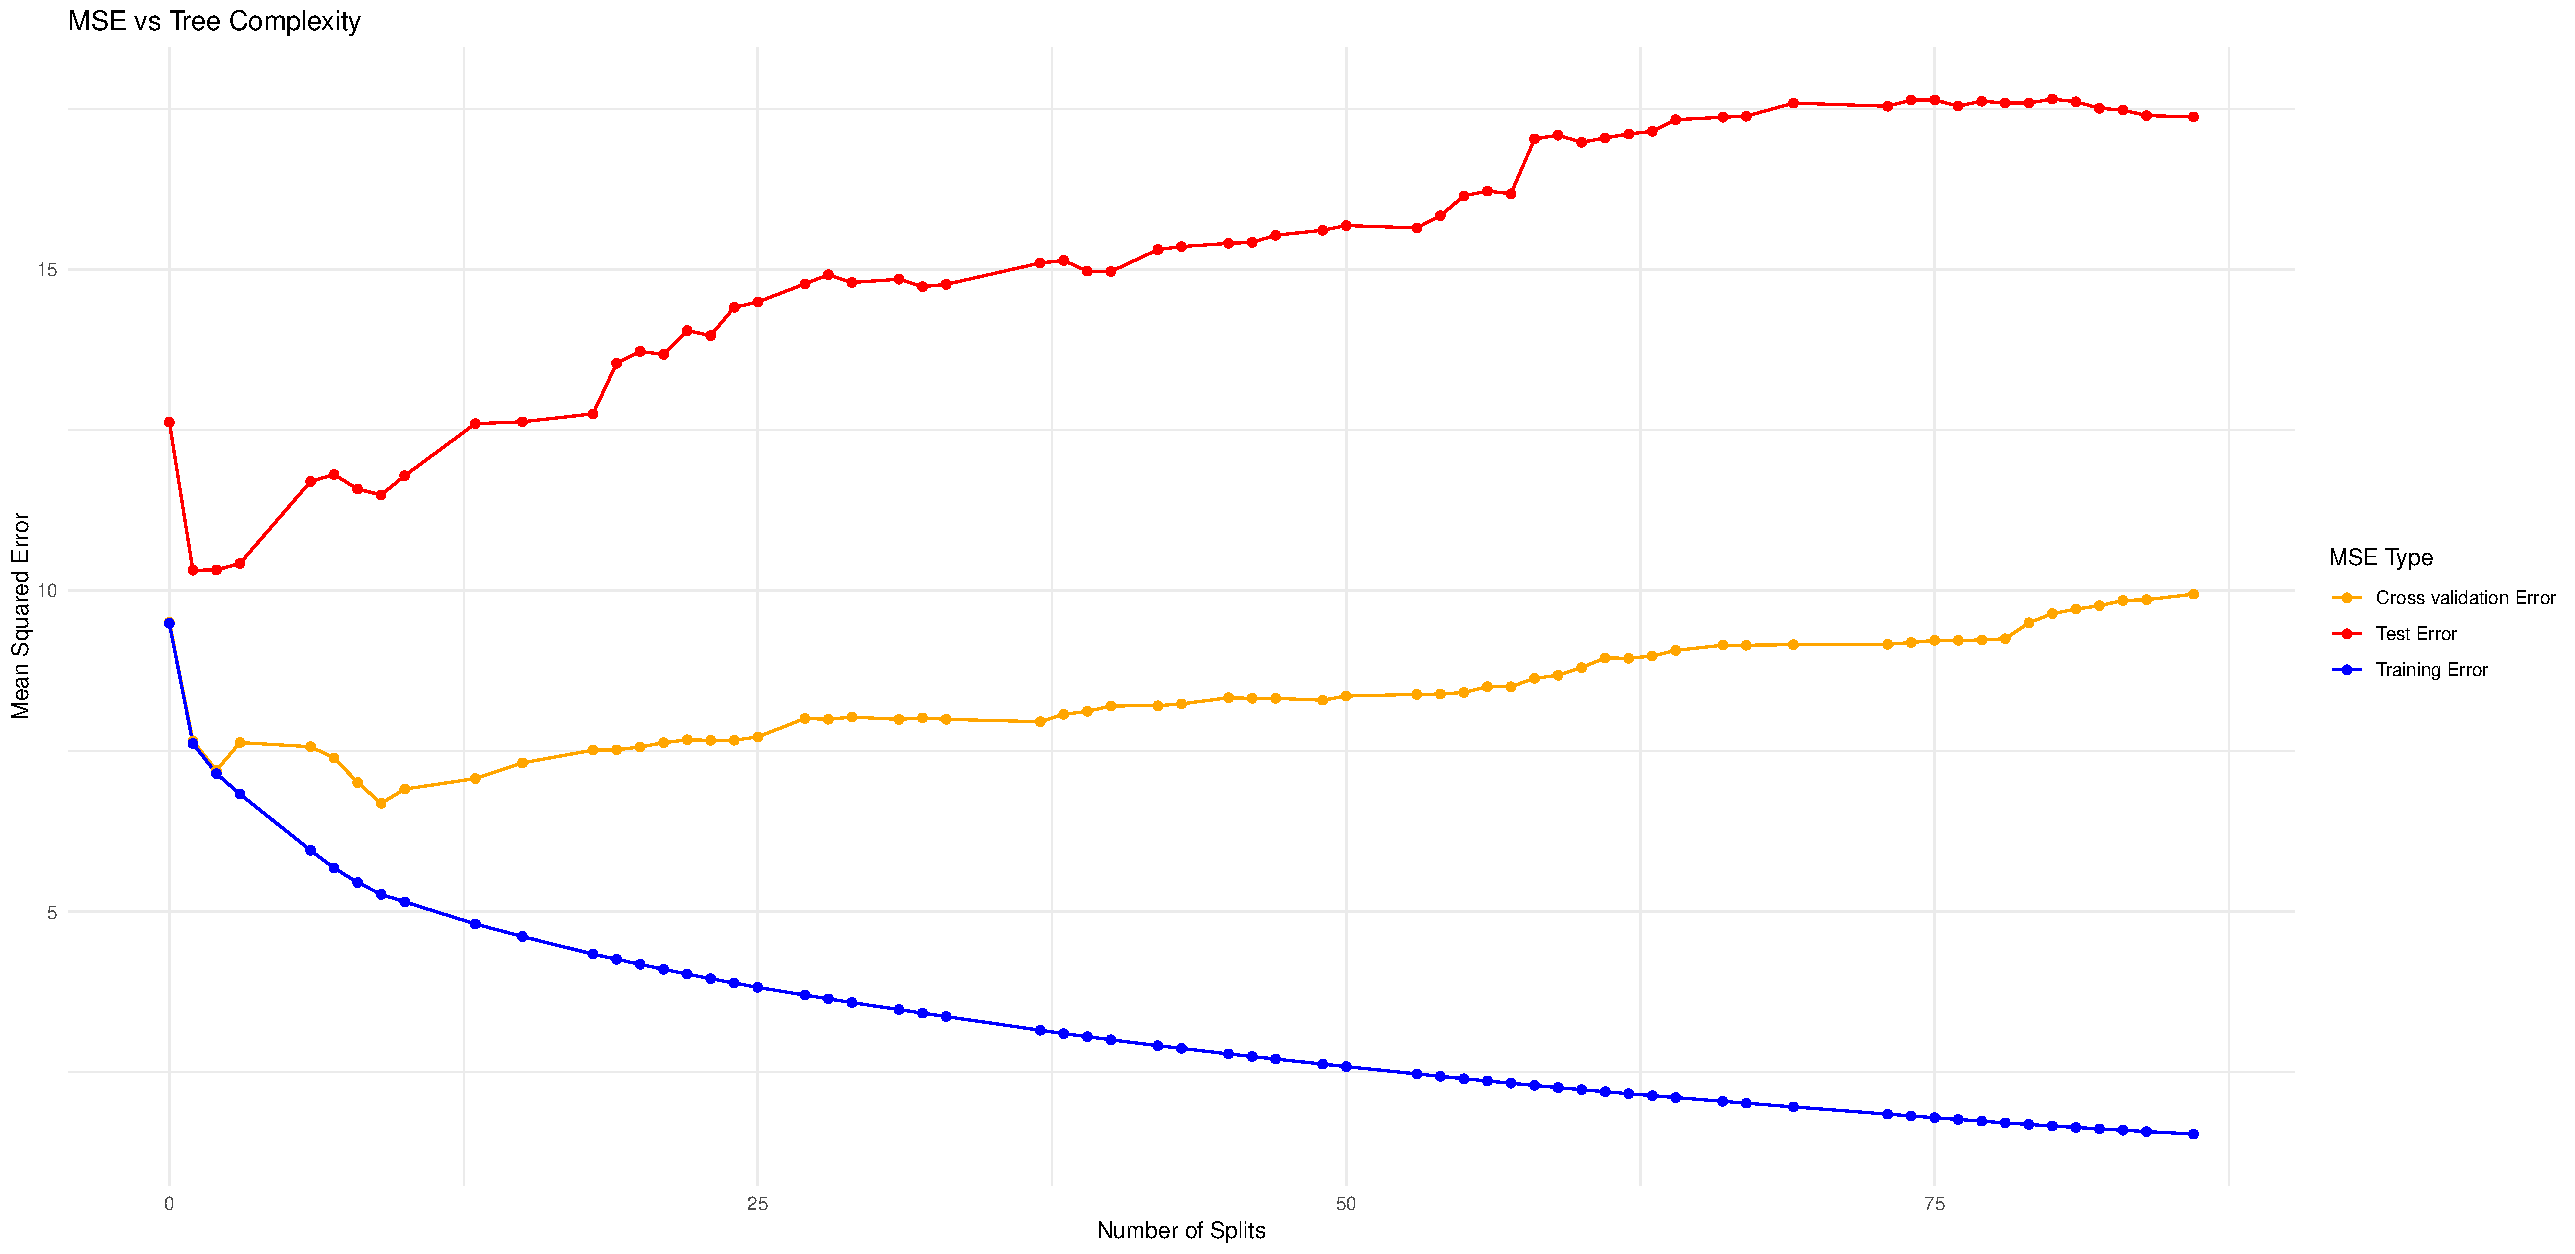
\includegraphics[scale=0.30]{triple_pruning_plot.pdf}
    \caption{Pruning finds the lowest Test error}
    \label{prune}
\end{figure}

Figure~\ref{prune} shows how the cross-validation error helps against overfitting as it does not decrease (almost) monotonically, but still overfits to a large extent. In this case, the optimal tree using cross-validation has 9 splits while the optimal tree evaluated on the test set has only one.

While it is clear that the tree is not overfitting it also is not very insightful. With only one split the simple tree is something a human could likely have done by hand.

\subsection{Comparing Linear Regression, Regression Trees, and BART}

After examining the regression trees performance, it is informative to compare it with linear regression and BART, this comparison provides insight into the strengths and weaknesses of different techniques for our dataset. Interestingly, even without any specific optimization to counter overfitting, linear regression outperforms the pruned regression tree by a significant margin. Perhaps trees excel only when strong interaction effects occour in the data.

Invoking Condorcet, I will also evaluate the BART model, using the default hyperparameters.

Table~\ref{big_comparison} presents the MSEs for each model. It is important to note that these results can vary depending on the specific data split into training and validation sets, as well as other random factors in the modelling process. However the single regression tree is typically outperformed by linear regression, and BART generally outperforms both.

\begin{wraptable}{r}{0.5\textwidth}
    \centering
    \begin{tabular}{| l | c | c |}
        \hline
        Model & Training MSE & Validation MSE \\
        \hline
        Tree  & 8.527        & 8.189          \\
        Regr  & 6.787        & 6.865          \\
        BART  & 5.777        & 6.523          \\
        \hline
    \end{tabular}
    \caption{MSE values for different models}
    \label{big_comparison}
\end{wraptable}

While BART demonstrates superior performance in terms of MSE, it comes with a significant trade-off in terms of interpretability. The ensemble nature of BART, combining predictions from hundreds of trees, makes it far less intuitive to understand compared to a single regression tree or a linear model.

The most obvious problem with simple regression trees is that they overfit almost immediately without providing much utility. It seems hard to imagine to be able to do only one split on a dataset this large, with over 30 variables. With a dataset where students who drink more alcohol score slightly lower on a test, a linear regression might incorporate this subtle trend, possibly slightly improving performance on the test set. If this effect is mere noise, the coefficient will not be too large and will not drive up the test error too much. In contrast, at least on this dataset, regression trees seem unable not to hyper-focus on an area, that turns out to typically, just be noise, resulting in just one single split generally being optimal. While the linear regression does not overfit with over a dozen coefficients the tree manages to overfit with just two splits.


\section{Conclusion}

The simulations in this paper highlighted the extremes where regression trees or linear regression are at their most powerful, and show how regression trees are adept at handling non-linear and interactive effects. Certainly there are situations in which each model beats the other.

The section on real world data highlights the importance of avoiding overfitting, both by splitting the data into separate sets. As well as by overfitting in harder to notice ways. And shows how Ensemble methods such as BART, while often losing most interpretability can achieve very impressive results. While the regression tree, at least on this dataset, tends to overfit rapidly. Although Regression trees certainly have their applications. As the simulations demonstrate, for highly non-linear data, even a simple tree can outperform linear regression by a significant margin.

While BART often outperforms linear regression, it sacrifices interpretability, which is a key advantage of both linear models and regression trees, only slightly outperforming linear regression in predictive ability.

Ultimately, the choice of model depends on the characteristics of the data. While one can always find datasets where trees outperform other models, determining the most appropriate method for a given task remains a critical area of research with many unanswered questions.

Because linear regression is used so much, it is an important area of research as even a small increase in our statistical sophistication or knowledge about when which model is superior will have large positive effects.

%\newpage

\bibliography{sources}

\end{document}